\chapter{Special Functions}

\newthought{Certain functions} arise frequently in discrete mathematics. 
Here is a catalog of some important ones.

\section{Floor and ceiling functions}
To begin with, the {\bfseries floor function} is a function from $\R$ to $\Z$ 
which assigns
to each real number $x$, the largest integer which is less than or equal to $x$.
We denote the floor function by $\lfloor x\rfloor$. So $\lfloor x\rfloor = n$
 means
$n\in \Z$ and  $n\leq x< n+1$. For example, $\lfloor 4.2 \rfloor = 4$, and
$\lfloor 7 \rfloor = 7$. Notice that for any integer $n$, $\lfloor n \rfloor = n$.
Be a little careful with negatives: $\lfloor \pi \rfloor = 3$, but 
 $\lfloor -\pi \rfloor = -4$.
A dual function is denoted $\lceil x\rceil$,
where $\lceil x\rceil = n$ means $n\in \Z$ and $n\geq x>n-1$. This is the
{\bfseries ceiling function}. For example, $\lceil 4.2 \rceil = 5$ and 
$\lceil -4.2 \rceil = -4$.
\begin{marginfigure}
%\includegraphics[width=1.2\textwidth]{Graphics/Floor_function_pgf.png} %from standalone:Floor_function_pgf.tex
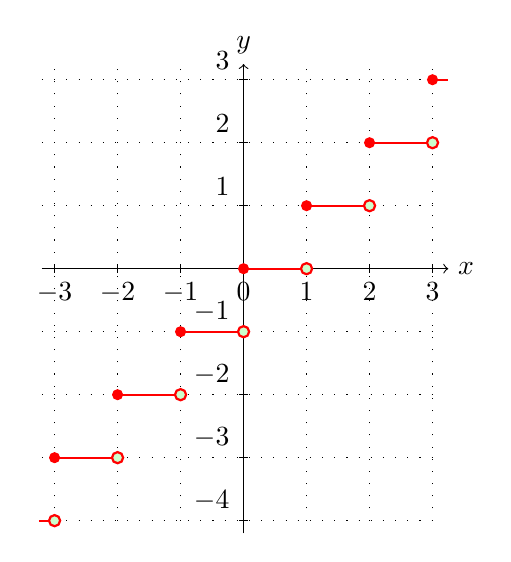
\begin{tikzpicture}[scale=0.80,
  font=\sffamily,
  source/.style={fill,circle,fill=red,inner sep=0.5mm},
  sink/.style={draw,circle,fill=green!20,inner sep=0.5mm},
  every node/.style={align=center}]

%draw axes and grid
    \draw[loosely dotted] (-3.2,-4) grid (3,3.2);
    \draw[->] (-3.2,0) -- (3.25,0) node[right] {$x$};
    \draw[->] (0,-4.2) -- (0,3.25) node[above] {$y$};
   
 %label and tic axes
    \foreach \x/\xtext in {-3/-3, -2/-2,-1/-1,0/0,1/1,2/2, 3/3}
    \draw[shift={(\x,0)}] (0pt,2pt) -- (0pt,-2pt) node[below] {$\xtext$};
    \foreach \y/\ytext in {-4/-4, -3/-3, -2/-2, -1/-1, 1/1, 2/2, 3/3}
    \draw[shift={(0,\y)}] (2pt,0pt) -- (-2pt,0pt) node[above left] {$\ytext$};

%draw jumps
  \foreach \x in {-3,-2,...,2} {
%     \draw[red,thick,dashed]  (\x,\x) node[sink] {} -- (\x,\x+1) node[source] {};
    \draw[red,thick]  (\x,\x) node[source] {} -- (\x+1,\x) node[sink] {}; }
%draw partial jumps
    \draw[red,thick]  (-3.25,-4.00) node {} -- (-3.00,-4.00) node[sink] {};
    \draw[red,thick]  (3.00,3.00) node[source] {} -- (3.25,3.00) node {};

    \end{tikzpicture}
\caption{Floor function}\label{fig:floor func}
\end{marginfigure}
The graph (in the college algebra sense!) of the floor function appears in
figure \ref{fig:floor func}.

\section{Fractional part}
The {\bfseries fractional part}\sidenote{This is the Mathematica and Wolfram/Alpha definition. Often, the Graham definition is used:
\[
 frac(x)=
  x - \lfloor x \rfloor, \text{ for all $x$}.
\]
} of a number $x\geq 0$ is denoted 
$frac(x)$ and equals
$x-\lfloor x\rfloor$. For numbers $x\geq 0$, the fractional part of $x$ is just 
what would be expected: the stuff following the decimal point.
 For example,
$frac(5.2) = 5.2 - \lfloor 5.2 \rfloor = 5.2 - 5 = 0.2$. 
When $x$ is negative its fractional part is defined to be 
$frac(x) = x-\lceil x\rceil$. Hence, we have
\[
 frac(x)=
  \begin{cases}
  x - \lfloor x \rfloor,\quad x \geq 0, \\
  x - \lceil x \rceil,\quad  x < 0.
  \end{cases} 
\]
\begin{marginfigure}
%\includegraphics[width=1.2\textwidth]{Graphics/Fractional_part_function_pgf.png} %from standalone:Fractional_part__function_pgf.tex
 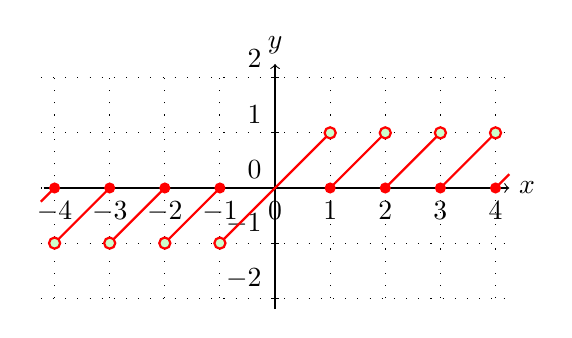
\begin{tikzpicture}[scale=0.70,
  font=\sffamily,
  source/.style={fill,circle,fill=red,inner sep=0.5mm},
  sink/.style={draw,circle,fill=green!20,inner sep=0.5mm},
  every node/.style={align=center}]

%draw axes and grid
    \draw[loosely dotted] (-4.25,-2) grid (4.2,2);
    \draw[->] (-4.2,0) -- (4.25,0) node[right] {$x$};
    \draw[->] (0,-2.2) -- (0,2.25) node[above] {$y$};
   
 %label and tic axes
    \foreach \x in {-4,-3,...,4}
     \draw[shift={(\x,0)}] (0pt,2pt) -- (0pt,-2pt) node[below] {$\x$};
     \foreach \y in {-2, -1,...,2}
    \draw[shift={(0,\y)}] (2pt,0pt) -- (-2pt,0pt) node[above left] {$\y$};

%draw saw teeth
  \foreach \x in {-4,-3,-2} {
     \draw[red,thick]  (\x,-1) node[sink] {} -- (\x+1,0) node[source] {};
%     \draw[red,thick,dashed]  (\x+1,-1) node[sink] {} -- (\x+1,0) node[source] {};
  }

  \draw[red,thick]  (-1,-1) node[sink] {} -- (1,1) node[sink] {};
%  \draw[red,thick,dashed]  (1,1) node[sink] {} -- (1,0) node[source] {};

  \foreach \x in {1,2,3} {
     \draw[red,thick]  (\x,0) node[source] {} -- (\x+1,1) node[sink] {};
%     \draw[red,thick,dashed]  (\x+1,0) node[source] {} -- (\x+1,1) node[sink] {};
  }
%draw partial teeth
    \draw[red,thick]  (-4.25,-0.25) node {} -- (-4,0) node[source] {};
%    \draw[red,thick,dashed]  (-4,0) node[source] {} -- (-4,-1) node[sink] {};
    \draw[red,thick]  (4,0) node[source] {} -- (4.25,0.25) node {};

\end{tikzpicture}

\caption{Fractional part function}\label{fig:frac part func}
\end{marginfigure}
For example, $frac(-5.2) = -5.2 - \lceil -5.2 \rceil = -5.2 - (-5) = -0.2$
In plain English, to determine the fractional part of a number $x$, take 
the stuff after the decimal point and keep the sign of the number.
The graph of the fractional part function is shown in figure \ref{fig:frac part func}.


\section{Integral part}
For any real
 number $x$
its {\bfseries integral part} is defined to be  $x-frac(x)$. 
\begin{marginfigure}
% \includegraphics[width=1.25\textwidth]{Graphics/Integral_part_function_pgf.png} %from standalone:Integral_part__function_pgf.tex
\begin{tikzpicture}[scale=0.85,
  font=\sffamily,
  source/.style={fill,circle,fill=red,inner sep=0.5mm},
  sink/.style={draw,circle,fill=green!20,inner sep=0.5mm},
  every node/.style={align=center}]

%draw axes and grid
    \draw[loosely dotted] (-3.2,-3.2) grid (3.2,3.2);
    \draw[->] (-3.2,0) -- (3.25,0) node[right] {$x$};
    \draw[->] (0,-4.2) -- (0,3.25) node[above] {$y$};
   
 %label and tic axes
    \foreach \x/\xtext in {-3/-3, -2/-2,-1/-1,0/0,1/1,2/2, 3/3}
    \draw[shift={(\x,0)}] (0pt,2pt) -- (0pt,-2pt) node[below] {$\xtext$};
    \foreach \y/\ytext in { -3/-3, -2/-2, -1/-1, 1/1, 2/2, 3/3}
    \draw[shift={(0,\y)}] (2pt,0pt) -- (-2pt,0pt) node[above left] {$\ytext$};

%draw jumps
  \foreach \x in {-3,-2} {
%     \draw[red,thick,dashed]  (\x,\x) node[source] {} -- (\x,\x+1) node[sink] {};
    \draw[red,thick]  (\x,\x+1) node[sink] {} -- (\x+1,\x+1) node[source] {}; }

% \draw[red,thick,dashed] (-1,-1) node[source] {} -- (-1,0) node[sink] {};
 \draw[red,thick] (-1,0) node[sink] {} -- (1,0) node[sink] {};

  \foreach \x in {1,2} {
%     \draw[red,thick,dashed]  (\x,\x-1) node[sink] {} -- (\x,\x) node[source] {};
    \draw[red,thick]  (\x,\x) node[source] {} -- (\x+1,\x) node[sink] {}; }

%%draw partial jumps
    \draw[red,thick]  (-3.25,-3.00)  -- (-3.00,-3.00) node[source] {};
%    \draw[red,thick,dashed]  (3,2) node[sink] {} -- (3,3) node[source] {};
    \draw[red,thick] (3,3) node[source] {} -- (3.25,3);

\end{tikzpicture}
 \caption{Integral part function}\label{fig:integral part func}
\end{marginfigure}
The integral part can equivalently be defined
by
\[
 \left[x\right]=
 \begin{cases}
  \lfloor x \rfloor, \quad x \geq 0, \\
  \lceil x \rceil, \quad x < 0.
 \end{cases}
\]
The integral part of $x$
 is denoted
by $[x]$, or, sometimes, by $int(x)$. In words, the integral part of $x$ is found by discarding everything
following the decimal (at least if we agree not to end decimals with
an infinite string of $9$'s such as $2.9999\cdots$). The graph of the integral part
function is displayed in figure \ref{fig:integral part func}.


\section{Power functions}
The {\bfseries power functions} are familiar from college algebra. They are
functions of the form $f(x) = x^2$, $f(x)=x^3$, $f(x)=x^4$, and so on.
By extension, $f(x) = x^a$, where $a$ is any constant greater than
or equal to $1$ will be called a power function. 

For any set $X$, the unit power function $1_{X}(x) = x$ for all $x\in X$ is called the
{\bfseries identity} function.

\section{Exponential functions}
Exchanging the roles of the variable and the constant in the power
functions leads to
a whole class of interesting functions, those of the form $f:\R\to \R$,
 where $f(x)=a^x$,
and $0<a$. Such a  function $f$ is called the {\bfseries base $a$ exponential
 function}. The
function is not very interesting when $a=1$. Also if $0<b<1$, then the function 
$\dl{g(x)=b^x={1\over f(x)}}$, where $f(x)=a^x$, and $\dl{a={1\over b}>1}$.
So we may focus on $a>1$. In fact the most important values for $a$ are $2,e$
 and $10$.
The number $e\approx 2.718281828459...$ is called the {\bfseries natural base}, but
that story belongs to calculus. Base $2$ is the usual base for computer science.
Engineers are most interested in base $10$, while mathematicians often use
the natural exponential function, $e^x$.%
\begin{marginfigure}
% \includegraphics[width=1.25\textwidth]{Graphics/Exponential_logarithm_functions_pgf.png} %from standalone:Exponential_logarithm_functions_pgf.tex
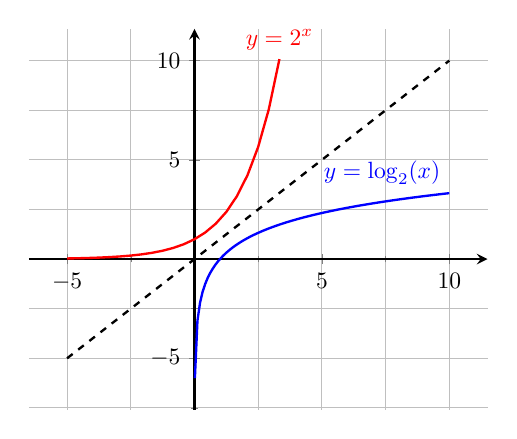
\begin{tikzpicture}[scale=0.85]
\pgfplotsset{every axis/.append style={line width=1pt}}
%draw axes and grid
%    \draw[loosely dotted] (-4.25,-2) grid (4.2,2);
%    \draw[->] (-4.2,0) -- (4.25,0) node[right] {$x$};
%    \draw[->] (0,-2.2) -- (0,2.25) node[above] {$y$};

\begin{axis}[grid=both, minor tick num=1,
          xmax=10,ymax=10,
          axis lines=middle,
          restrict y to domain=-7:12,
          enlargelimits]
%\addplot[orange,domain=1/2^6:2.25,samples=100]  {pow(e,x)} node[above left]{$y=e^x$};
\addplot[red]  {pow(2,x)} node[above]{$y=2^x$};
\addplot[blue,domain=1/2^6:10,samples=100]  {log2(x)} node[above left] {$y=\log_2(x)$};
%\addplot[,domain=1/2^6:10,samples=100]  {ln(x)} node[below left] {$y=\ln(x)$};
\addplot[black,dashed,domain=-5:10] {x};
\end{axis}
\end{tikzpicture}
 \caption{$2^x$ and $\log_2(x)$ functions}\label{fig:exp_2 log_2 funcs}
\end{marginfigure}%

\section{Logarithmic functions}
By graphing the function $f:\R \to (0,\infty)$ defined by $y=f(x)=e^x$ we
 can see that it is 
bijective. We denote the inverse function $f^{-1}(x)$ by $\ln x$ and call it the 
{\bfseries natural log
function}. Since these are inverse functions we have 
\[
 e^{\ln a}=a, \forall a>0 \text{~and~} \ln (e^b) = b, \forall b\in \R.
\]
As a consequence $a^x=(e^{\ln a})^x=e^{(\ln a) \cdot x}=e^{x\ln a}$ is
 determined as the
 composition of 
$y=(\ln a) x$ by the natural exponential function. 
So every exponential function is invertible with inverse denoted as $\log_a x$, 
the
 {\bfseries base $a$ logarithmic
function}. Besides the natural log, $\ln x$, we often write $\lg x$ for
 the base $2$
 logarithmic function, and
$\log x$ with no subscript to denote the base $10$ logarithmic function. 

\section{Laws of logarithms}
The basic facts needed for manipulating exponential and logarithmic functions
are the laws of exponents.
\begin{thm}[Laws of Exponents] 
 For $a,b,c\in \R$, 
 $a^{b+c}=a^b\cdot a^c$, $a^{bc}=(a^b)^c$
 and $a^cb^c=(ab)^c$.
\end{thm}
From the laws of exponents, we can derive the
\begin{thm}[Laws of Logarithms] 
 For $a, b,c>0,\log_a {bc}=\log_a b + \log_a c,$ and
 $\log_a (b^c)=c\log_a b$.
\end{thm} 
\begin{proof}
 We rely on the fact that all exponential and logarithmic 
 functions are one-to-one. Hence, we have that
 \[
  a^{\log_a bc} = bc = a^{\log_a b}a^{\log_a c}=a^{\log_a b +\log_a c},
 \]
 implies 
 \[
  \log_a bc = \log_a b + \log_a c.
 \] 
 Similarly, the second identity follows from
 \[
  a^{\log_a b^c} = b^c = (a^{\log_a b})^c=a^{c\log_a b}.
 \]
\end{proof}

Notice that $\displaystyle{\log_a \frac{1}{b}= \log_a b^{-1} = -\log_a b}$.

Calculators typically have buttons for logs base $e$ and base $10$.
If $\log_a b$ is needed for a base different from $e$ and $10$,
it can be computed in a roundabout way. Suppose we need
to find $c = \log_a b$. In other words, we need the number $c$
such that $a^c=b$. Taking the $\ln$ of both sides of that equation
we get
\begin{align*}
 a^c &= b \\
 \ln\left(a^c\right) &= \ln b \\
 c\ln a &= \ln b \\
 c &= {{\ln b}\over{\ln a}}
\end{align*}

Hence, we have the general relation between logarithms as follows.
\begin{corollary}
 So, we have $\log_a(x) = {{\ln x}\over{\ln a}}$.
\end{corollary}

\begin{exmp}
 For example, we see that
$log_2 {100} = {{\ln 100}\over{\ln 2}}\approx 6.643856$.
\end{exmp}

\clearpage




\section{Exercises}
\begin{exer}
In words, $\lfloor{x}\rfloor$ is the largest integer less than or equal to $x$. \textbf{Complete the sentence}: 
\emph{In words,$\lceil{x}\rceil$ is the smallest $\dots\dots$} .
\end{exer}

\begin{exer}
Draw a (college algebra) graph of $f(x) = \lceil x \rceil$.
\end{exer}

\begin{exer}
 Draw a (college algebra) graph of $f(x) = \lfloor 2x-1 \rfloor$.

\end{exer}

\begin{exer}
 Draw a (college algebra) graph of $f(x) = 2\lfloor x-1\rfloor$.

\end{exer}

\begin{exer}
 Let $f(x) = 18x$ and let $\displaystyle g(x) = \frac{x^3}{2}$. Sketch the graphs of $f$ and $g$ for $x\geq 1$ on the same set of axes. Notice that the graph $g$ is lower then the graph of $f$ when $x=1$, 
but it is above the graph of $f$ when $x=9$. Where does $g$ cross the graph of $f$ (in other words, where does $g$ catch up with $f$)?

\end{exer}

\begin{exer}
 Let $f(x) = 4x^5$ and let $g(x) = 2^x$. For values of $x\geq 1$ it appears that the graph of $g$ is lower than the graph of $f$.
Does $g$ ever catch up with $f$, or does $f$ always stay ahead of $g$?

\end{exer}

\begin{exer}
 The $x^y$ button on your calculator is broken. Show how can you approximate $2^{\sqrt{2}}$ with your calculator anyhow.
\end{exer}

\clearpage

\section{Problems}

\begin{prob}
Write $\displaystyle \frac{5}{2}\ln{5} - 4 \ln{3}$ as a single logarithm.
\end{prob}

\begin{prob}
 Draw the college algebra style graph of $f(x) = e^{x+3} -1$.
\end{prob}

\begin{prob}
Let $f(x) = 2x^3$ and $g(x) = 3^x$. Notice that $f(1) < g(1)$ and $f(2) = g(2)$. Does $g$ ever 
catch up with $f$ again, or does $f$ always stay ahead of $g$?
\end{prob}

\begin{prob}
Write $\lg 1+ \lg 2 + \lg 3 + \lg 4 + \lg 5 + \lg 6$ as a single logarithm.
\end{prob}

\begin{prob}
Write $\displaystyle \sum_{k=1}^{n} \lg{n}$ as a single logarithm.
\end{prob}